\documentclass[a4paper, 12pt]{article}
\usepackage[utf8]{inputenc}
\usepackage{myshortcuts}
\usepackage{a4wide}
\usepackage{csquotes}
% \usepackage{hyperref}
\usepackage[english]{babel}
\usepackage[labelfont=bf]{caption}
\usepackage[style=mla,backend=biber]{biblatex}

\addbibresource{mysources.bib}


\title{
\textbf{Mathematics Internal Assessment}\\
\bigskip
Is this a good title for the IA?
}
\author{Jingjie YANG}
\date{}

\begin{document}
\maketitle

\section{Introduction}
If a large, porous stone is immersed in water for a long time, what is the probability that its centre is wetted? In 1957, Broadbent and Hammersley \autocite*[693]{broadbent_hammersley_1957} formulated a simple stochastic model for this situation, which in two dimensions amounts to a large grid of channels. More specifically, we consider the graph $G = (V, E)$, where the set of vertices $V$ is the square lattice $\Z^2$, and all the edges that connect two neighbouring points $A$ and $B$ on the square lattice, i.e. $\abs{A_x - B_x} + \abs{A_y - B_y} = 1$, constitute the set of edges $E$. We then choose a certain $p \in [0, 1]$, and for each edge (alternatively called \textit{bond}) $e$ in $E$, we declare $e$ to be \textit{open} with probability $p$, and \textit{closed} otherwise with probability $1 - p$ independently of the states of other edges. This model is known as Bernoulli bond percolation.

\begin{figure}[!hb]
    \centering
    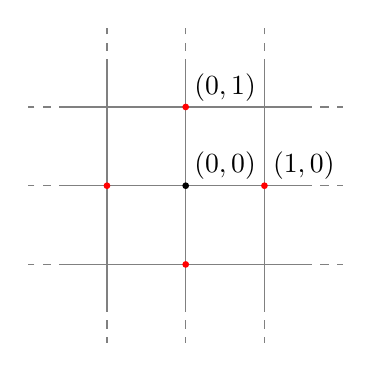
\begin{tikzpicture}
        \foreach \i in {-1, 0, 1} {
            \draw[gray] (-1.5, \i) -- (1.5, \i);
            \draw[gray] (\i, -1.5) -- (\i, 1.5);
            
            \draw[gray, dashed] (-1.5, \i) -- (-2.0, \i);
            \draw[gray, dashed] (\i, -1.5) -- (\i, -2.0);
            \draw[gray, dashed] (1.5, \i) -- (2.0, \i);
            \draw[gray, dashed] (\i, 1.5) -- (\i, 2.0);
        }
        \node at (0.5, 0.25) {$(0, 0)$};
        \node at (1.5, 0.25) {$(1, 0)$};
        \node at (0.5, 1.25) {$(0, 1)$};
        
        \filldraw (0, 0) circle (1pt);
        \filldraw[red] (0, +1) circle (1pt);
        \filldraw[red] (0, -1) circle (1pt);
        \filldraw[red] (-1, 0) circle (1pt);
        \filldraw[red] (+1, 0) circle (1pt);
    \end{tikzpicture}
    \caption{The origin (black) and its 4 neighbours (red) on the square lattice}
    \label{fig:square_lattice}
\end{figure}

The edges represent the inner passageways of the stone, where open edges let water through and closed ones block the flow; water reaches the centre of the stone if and only if the origin is in a connected component of open edges touching the boundary of the stone. In addition, it is not unreasonable to assume that the fine structure of the interior channels is on a negligible scale compared to the overall size of the stone. We are then interested in knowing whether the origin belongs to a connected component of infinitely many vertices, also called an \textit{infinite cluster}. 

Apart from $p = 0$ where the stone is entirely impermeable, and $p = 1$ where water flows surely past the origin, to have an idea of how the model behaves at other nontrivial values of $p$, we can contemplate computer simulations of a finite section of the square lattice:

\begin{figure}[!h]
    \centering
    \caption{Percolation realisations on a $16 \times 16$ section of $\Z^2$ for 3 different values of $p$}
    \label{fig:3_realisations}
    \minipage{0.32\textwidth}
    \centering
    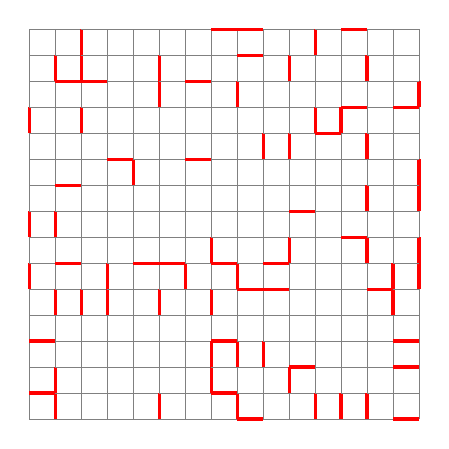
\begin{tikzpicture}
        \def\p{0.2}
        \foreach \x in {0,0.33,...,4.63} {
            \foreach \y in {0,0.33,...,4.63} {
                \pgfmathparse{rnd}
                \ifdim\pgfmathresult pt < \p pt\relax 
                    \draw[red, very thick] (\x, \y) -- (\x, \y + 0.33);
                \else
                    \draw[gray] (\x, \y) -- (\x, \y + 0.33);
                \fi 
                \pgfmathparse{rnd}
                \ifdim\pgfmathresult pt < \p pt\relax
                    \draw[red, very thick] (\x, \y) -- (\x + 0.33, \y);
                \else
                    \draw[gray] (\x, \y) -- (\x + 0.33, \y);
                \fi 
            }
            \pgfmathparse{rnd}
            \ifdim\pgfmathresult pt < \p pt\relax
                \draw[red, very thick] (\x, 4.95) -- (\x + 0.33, 4.95);
            \else
                \draw[gray] (\x, 4.95) -- (\x + 0.33, 4.95);
            \fi
            \pgfmathparse{rnd}
            \ifdim\pgfmathresult pt < \p pt\relax
                \draw[red, very thick] (4.95, \x) -- (4.95, \x + 0.33);
            \else
                \draw[gray] (4.95, \x) -- (4.95, \x + 0.33);
            \fi
        }
    \end{tikzpicture}
    \caption*{$p = 0.2$}
    \endminipage\hfill
    \minipage{0.32\textwidth}
    \centering
    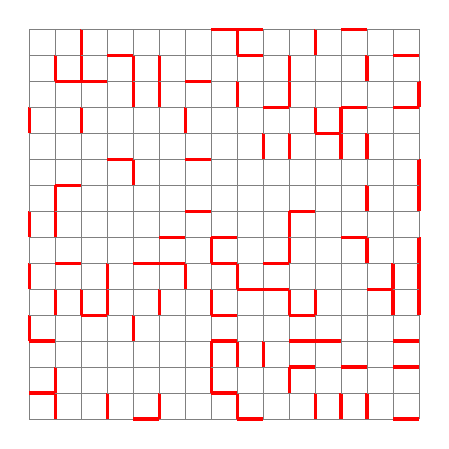
\begin{tikzpicture}
        \def\p{0.3}
        \foreach \x in {0,0.33,...,4.63} {
            \foreach \y in {0,0.33,...,4.63} {
                \pgfmathparse{rnd}
                \ifdim\pgfmathresult pt < \p pt\relax 
                    \draw[red, very thick] (\x, \y) -- (\x, \y + 0.33);
                \else
                    \draw[gray] (\x, \y) -- (\x, \y + 0.33);
                \fi 
                \pgfmathparse{rnd}
                \ifdim\pgfmathresult pt < \p pt\relax
                    \draw[red, very thick] (\x, \y) -- (\x + 0.33, \y);
                \else
                    \draw[gray] (\x, \y) -- (\x + 0.33, \y);
                \fi 
            }
            \pgfmathparse{rnd}
            \ifdim\pgfmathresult pt < \p pt\relax
                \draw[red, very thick] (\x, 4.95) -- (\x + 0.33, 4.95);
            \else
                \draw[gray] (\x, 4.95) -- (\x + 0.33, 4.95);
            \fi
            \pgfmathparse{rnd}
            \ifdim\pgfmathresult pt < \p pt\relax
                \draw[red, very thick] (4.95, \x) -- (4.95, \x + 0.33);
            \else
                \draw[gray] (4.95, \x) -- (4.95, \x + 0.33);
            \fi
        }
    \end{tikzpicture}
    \caption*{$p = 0.3$}
    \endminipage\hfill
    \minipage{0.32\textwidth}
    \centering
    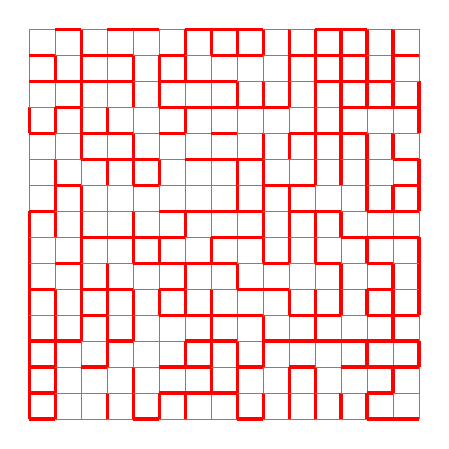
\begin{tikzpicture}
        \def\p{0.6}
        \foreach \x in {0,0.33,...,4.63} {
            \foreach \y in {0,0.33,...,4.63} {
                \pgfmathparse{rnd}
                \ifdim\pgfmathresult pt < \p pt\relax 
                    \draw[red, very thick] (\x, \y) -- (\x, \y + 0.33);
                \else
                    \draw[gray] (\x, \y) -- (\x, \y + 0.33);
                \fi 
                \pgfmathparse{rnd}
                \ifdim\pgfmathresult pt < \p pt\relax
                    \draw[red, very thick] (\x, \y) -- (\x + 0.33, \y);
                \else
                    \draw[gray] (\x, \y) -- (\x + 0.33, \y);
                \fi 
            }
            \pgfmathparse{rnd}
            \ifdim\pgfmathresult pt < \p pt\relax
                \draw[red, very thick] (\x, 4.95) -- (\x + 0.33, 4.95);
            \else
                \draw[gray] (\x, 4.95) -- (\x + 0.33, 4.95);
            \fi
            \pgfmathparse{rnd}
            \ifdim\pgfmathresult pt < \p pt\relax
                \draw[red, very thick] (4.95, \x) -- (4.95, \x + 0.33);
            \else
                \draw[gray] (4.95, \x) -- (4.95, \x + 0.33);
            \fi
        }
    \end{tikzpicture}
    \caption*{$p = 0.6$}
    \endminipage\hfill
\end{figure}
\break 

Readers with good eyesight may bother to check that for $p = 0.6$, there is a path of open edges (in red) connecting the left and right sides, whereas such is not the case for $p = 0.2$ and $p = 0.3$ where the connected components are isolated. Is there a value of the parameter $p$ at which infinite clusters emerge? Can we compute this critical value of $p$? Is the critical value different for the cubic lattice $\Z^3$?

What is described above forms the basis of percolation theory. Since its birth in 1957 due to Broandbent and Hammersley \autocite*[693]{broadbent_hammersley_1957}, the field has attracted pure mathematicians and scientists from myriad domains. Despite its simplicity, the percolation model accounts for the behaviour of many natural systems --- ranging from the flow of fluids through a disordered porous medium and ferromagnetism of materials to the spread of forest fires and epidemics \autocite[60]{gennes_2000}. Nevertheless, the first major mathematical result was not announced until only some twenty years later: in 1980, Kesten \autocite*[41]{kesten_1980} completed Harris and Lindley's \autocite*[13]{harris_lindley_1960} 1960 work to prove that the critical probability on the square lattice is equal to $\frac{1}{2}$. In the last two decades, there has been remarkable progress in our understanding of two-dimensional percolation due to Smirnov's \autocite*[239]{smirnov_2001} proof of the conformal invariance on the hexagonal lattice, for which he received the Fields Medal in 2010.

To answer the questions raised above about the existence of the critical probability on the square and cubic lattices, we will firstly acquaint ourselves with a few notions in probability to allow for a rigorous discussion of the subject.

\section{Probabilistic Preliminaries}
We shall not get burdened by the measure-theoretic details about the probability space, but to avoid juggling with infinities in the model, some formal definitions are required.

\begin{defn}\label{defn:outcome_and_event}
We call a percolation an \textit{outcome}. For example, the leftmost panel of Figure~\ref{fig:3_realisations} shows an outcome when $p = 0.2$. An \textit{event} is a set of zero or more outcomes, and depends finitely many edges. We say an event \textit{occurs} if the outcome belongs to the event.
\end{defn}

\begin{ex}\label{ex:cluster_of_size_n}
For positive integer $n$, we define the event
\[
\{\abs{C} \geq n\}
= \{\text{the cluster contains a vertex at distance } n \text{ of } O\}.
\]
where $O$ refers to the origin and $\abs{C}$ denotes the size of the cluster containing $O$.
\end{ex}

As usual, the probabilities of any events $A$ and $B$ satisfy the following:
\begin{itemize}
    \item $P(A \cup B) = P(A) + P(B) - P(A \cap B)$;
    \item $A$ and $B$ are \textit{independent} if and only if $P(A \cap B) = P(A) P(B)$;
    \item $0 \leq P(A) \leq 1$ --- in particular, $P(\varnothing) = 0$.
\end{itemize}

\begin{lem}\label{lem:event_subseteq}
If the occurrence of event $A$ implies the occurrence of event $B$, then $$P(A) \leq P(B).$$
\end{lem}
\begin{proof}
By Definition~\ref{defn:outcome_and_event}, we see that $A$ and $B$ are two sets of outcomes where, for all $\omega \in A$, we also have $\omega \in B$. Hence $A \subseteq B$, and 
\begin{align*}
    P(B) 
    &= P(A \cup (B \setminus A))\\
    &= P(A) + P(B \setminus A) - P(A \cap (B \setminus A))\\
    &\geq P(A)
\end{align*}
since $A \cap (B \setminus A) = \varnothing$ and $P(B \setminus A) \geq 0$.
\end{proof}

\begin{cor}\label{cor:inf_cluster}
Using the definition from Example~\ref{ex:cluster_of_size_n}, for positive integers $m$ and $n$, if $n > m$, we have $\{\abs{C} \geq n\} \subseteq \{\abs{C} \geq m\}$ and hence $P(\abs{C} = n) \leq P(\abs{C} = m)$. We then define
\[
\theta(p) 
= P(\abs{C} = \infty)
= \lim_{n \to \infty} P(\text{the cluster contains a vertex at distance } n \text{ of } O).
\]
\end{cor}

\section{Critical Value on the Square Lattice}
To start with, we want to know for which values of $p$ there is no infinite cluster on the square lattice, i.e., $\theta(p) = 0$.

\begin{prop}
test test
\end{prop}

\begin{lem}[Boole's inequality]\label{lem:union_bound}
$n \in \N, P(A_1 \cup A_2 \cup \cdots \cup A_n) \leq P(A_1) + P(A_2) + \cdots + P(A_n)$
\end{lem}
\begin{proof}[Proof]
We proceed by induction on $n$. Let $\mathcal{P}(n): P(\bigcup_{i = 1}^n A_i) \leq \sum_{i = 1}^n P(A_i)$ for  $n \in \N$.
\begin{description}
\item \textit{Base case.} We have $P(A_1) \leq P(A_1)$, and hence $\mathcal{P}(1)$ is true.
\item \textit{Inductive step.} Assume that $\mathcal{P}(k)$ is true for a certain $k \in \N$; show that $\mathcal{P}(k + 1)$ is true.
We use the associative property of the union operation:
\begin{align*}
    P(\bigcup_{i = 1}^{k + 1} A_i) 
    &= P(\bigcup_{i = 1}^{k} A_i \cup A_{k + 1})\\
    &= P(\bigcup_{i = 1}^{k} A_i) + P(A_{k + 1}) - P(\bigcup_{i = 1}^{k} A_i \cap A_{k + 1})\\
    &\leq \sum_{i = 1}^k P(A_i) + P(A_{k + 1}) - P(\bigcup_{i = 1}^{k} A_i \cap A_{k + 1})\\
\end{align*}
Since $P(\bigcup_{i = 1}^{k} A_i \cap A_{k + 1}) \geq 0$, we can conclude that $P(\bigcup_{i = 1}^{k + 1} A_i) \leq \sum_{i = 1}^{k + 1} P(A_i)$.
\end{description}
By the principle of mathematical induction, $\mathcal{P}(n)$ is true for any $n \in \N$.
\end{proof}

\section{Critical Value on the Cubic Lattice}

\section{Conclusion}
\begin{quotation}
``Quite apart from the fact that percolation theory had its origin in an honest applied problem, it is a source of fascinating problems of the best kind a mathematician can wish for: problems which are easy to state with a minimum of preparation, but whose solutions are (apparently) difficult and require new methods.''
\end{quotation}

\nocite{*}
\printbibliography

\end{document}
